%%%%%%%%%%%%%%%%%%%%%%%%%%%%%%%%%%%%%%%%%%%%%%%%%%%%%%%%%%%%%%%%%%%
%                                                                 %
%                            CHAPTER FOUR                         %
%                                                                 %
%%%%%%%%%%%%%%%%%%%%%%%%%%%%%%%%%%%%%%%%%%%%%%%%%%%%%%%%%%%%%%%%%%%

\chapter{SCALABLE PARALLEL MESH ADAPTATION}
\label{chap:parallel}

\section{Definition}

What does it mean to scale well.

\begin{equation} \label{eq:big-o-scale}
t = O\left(\frac{N}{P}\lg(P)\right)
\end{equation}

A list of requirements for scalability:

\begin{enumerate}
\item Never collect data of size $O(P)$ on one processor
\end{enumerate}

\section{Scalable Non-Blocking Collectives}
\label{sec:nbx}

Half of the PCU paper goes here; the key algorithms
that got PHASTA to really large core counts and
that PETSc/Trilinos are still catching up on for
matrix assembly.

\section{Entity-Level Communication}
\label{sec:dist}

Something which both PCU and Omega\_h do is simulate
mesh entities sending messages to each other, while
doing this much more efficiently than the naive approach.

\section{Remotes and Owners}

Explain remote copies and owners, and how they become
part of the two structures from \ref{chap:struct}.

\section{Migration}

Both the PUMI/APF and Omega\_h migration algorithms
are quite different from what has been published for FMDB,
and they are essentially what it means for a mesh
data structure to be parallel.

\section{Ghosting}

As with migration, describe what is done in both PUMI/APF
and Omega\_h.

\section{Parallel Cavity Operations}

\subsection{Dynamic Migration}
\label{sec:cavity_operator}

The PUMI/APF ``Cavity Operator" system that supports MeshAdapt.

\subsection{Independent Sets}
\label{sec:indset}

{\color{red} this is from the rejected full-paper submission to IMR 2016}

\subsubsection{Selection of a Set}

At each pass during mesh adaptation, we select a set of mesh modifications
whose affected cavities do not overlap (do not share elements) to apply.
This allows us to execute each modification using fine-grained parallelism.
Such an approach was suggested for GPU use by Pande et al. \cite{pandea2015gpu},
although their implementation computed the independent set on the CPU.
It is also already used in MPI-only adaptation codes \cite{de1999parallel}
during coarsening to prevent a chain of overlapping edge collapses
from removing too many mesh elements.

One can view this as a graph independent set problem, with a graph whose
graph nodes are possible modifications around certain key entities
and the graph edges represent an overlap between their cavities,
in our case meaning the key entities are adjacent to a common element.

We have either vertices or edges as the key entities, and either
triangles or tetrahedra for elements.
Fast algorithms can construct the graph of keys that are adjacent
to a common element, which we use as the basis for our conflict graph.
At the beginning of each pass, threshold and quality logic results
in each key entity being annotated as either being a candidate or
not, and if a candidate it is annotated with its output cavity quality.
We would like to resolve conflicts in a way that prefers ``better" mesh
modifications, which in this case is defined by output quality.

In 1986, Luby presented a highly parallelizable algorithm
for finding maximal independent sets of graphs \cite{luby1986simple}.
A maxim\emph{al} independent set is simply one that cannot be improved by
adding more graph nodes to it, as opposed to a maxim\emph{um} independent
set which is NP-hard to find and has the most graph nodes of any
possible independent set.
The structure of Luby's algorithm that we preserve is that it is iterative,
and at each iteration graph nodes which are local maxima of some function
are added to the independent set.
Each vertex can, in parallel, determine whether its function value is
less than that of its neighbors, and alter its own state (whether or not it is in the set)
with confidence that no neighbor will make an inconsistent decision.
Luby's original algorithm assigned random integers to each graph node
at each iteration, having no more information than the graph connectivity as input.

\begin{algorithm}
 \LinesNumbered
 \SetKwInOut{Input}{input}\SetKwInOut{Output}{output}
 \SetKwData{Xadj}{xadj}\SetKwData{Adj}{adj}
 \SetKwData{In}{IN}\SetKwData{Out}{NOT\_IN}\SetKwData{Unknown}{UNKNOWN}
 \SetKwData{OldState}{old\_state}\SetKwData{NewState}{new\_state}
 \SetKwData{Begin}{begin}\SetKwData{End}{end}
 \SetKwData{Quality}{quality}\SetKwData{Vqual}{v\_qual}\SetKwData{Uqual}{u\_qual}
 \SetKwData{Global}{global}
 \Input{Conflict graph $G=(V,E)$ represented by $n$, \Xadj and \Adj}
 \Input{Current vertex state in \OldState (entries are either \In, \Out, or \Unknown)}
 \Input{Quality measure for each graph vertex in \Quality}
 \Input{Unique graph node IDs in \Global}
 \Output{Updated vertex state in \NewState}
 \For(\tcp*[f]{shared memory parallel for loop}){$v \gets 0$ \KwTo $n-1$}{
   \If{\OldState$[v] \neq$\Unknown}{
     \Return\;
   }
   \Begin $\gets$ \Xadj $[v]$\;
   \End $\gets$ \Xadj $[v + 1]$\;
   \tcp{vertices adjacent to chosen ones are rejected}
   \For{$j \gets $\Begin \KwTo \End$-1$}{
     $u \gets$\Adj$[j]$\;
     \If{\OldState$[u] =$\In}{
       \NewState$[v] \gets$\Out\;
       \Return\;
     }
   }
   \tcp{check if vertex is local maximum}
   \Vqual$\gets$\Quality$[v]$\;
   \For{$j \gets $\Begin \KwTo \End$-1$}{
     $u \gets$\Adj$[j]$\;
     \tcp{neighbor was rejected, ignore its presence}
     \lIf{\OldState$[u] =$\Out}{
       continue to next $j$
     }
     \Uqual$\gets$\Quality$[u]$\;
     \tcp{neighbor has higher quality}
     \lIf{\Uqual$>$\Vqual}{
       \Return
     }
     \tcp{neighbor has equal quality, tiebreaker by global ID}
     \lIf{$($\Uqual$=$\Vqual$)$ {\bf and } $($\Global$[u]>$\Global$[v])$}{
       \Return
     }
   }
   \tcp{only local maxima reach this line}
   \NewState$[v] \gets$\In\;
 }
 \caption{One iteration of independent set selection}
 \label{alg:indset}
\end{algorithm}

Instead of local maxima of random numbers, we find local maxima of
output quality.
Our modified Luby iteration is listed in full detail
as Algorithm \ref{alg:indset}.
Its parallel \texttt{for} loop will have its iterations scheduled by the
current runtime (CUDA, OpenMP, etc.) onto the available hardware threads.
In the extreme case, there may be enough threads for all iterations
to execute simultaneously.
Of key importance in programming for shared memory is
the elimination of read and write contention between threads.
All arrays involved are either read-only or write-only,
and the latter (\texttt{new\_state}) has each entry written by one
thread only, by aligning its writes with the iterations
of the parallel \texttt{for} loop.

\begin{figure}[t]\vspace*{4pt}
\centerline{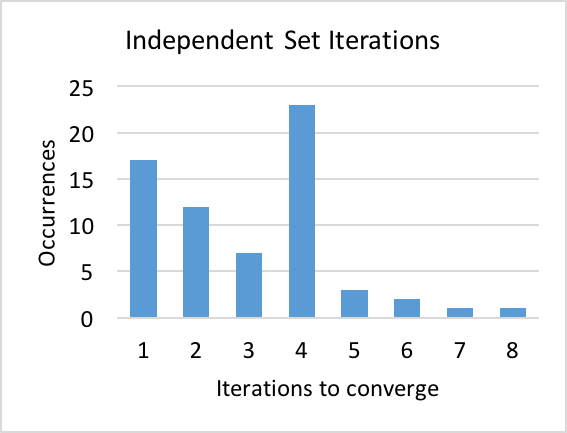
\includegraphics[width=0.3\textwidth]{indset_iters.png}}
\caption{Independent set convergence histogram}\vspace*{-6pt}
\label{fig:indset_conv}
\end{figure}

The proof for the time complexity of Luby's original algorithm
relied on probability theory and changing
the graph node numbers at each iteration \cite{luby1986simple}.
In our algorithm, the number of iterations is bounded by the
length of the longest path in the conflict graph whose nodes have monotonic
quality values.
Although it may be theoretically possible to construct pathological
meshes where this path length grows proportional to the number of elements,
in practice such paths are short.
Figure \ref{fig:indset_conv} shows a histogram of the number of
iterations required to find a maximal independent set during execution
of a typical Omega\_h mesh adaptation.
The algorithm terminates in fewer than ten iterations in all cases,
typically requiring about four iterations.

Finally, note that in line 20 of Algorithm \ref{alg:indset} we
compare graph node global IDs in the case of equal quality values.
Ties could otherwise cause the algorithm to deadlock, and we
prefer a deterministic resolution.
Thus in some cases the output is affected by the global ID values,
however this does not mean it is ordering-dependent because
we update global ID values in a way that is independent
of the local ordering of entities.

\subsubsection{Ghosting for Set Selection}

For distributed memory machines, we implement MPI parallelism
with the help of a generalized ``migration" mechanism.
Migration redistributes the copies of the mesh entities
across MPI ranks \cite{ibanez2015pumi}.
Each MPI rank specifies which entities it requires in the new
partition, using references to entities in the existing 
partition.
Multiple MPI ranks may request the same mesh entity, which
is the underlying mechanism to support ghost layers,
since even mesh elements may be requested by multiple ranks.
By using MPI 3.0 features including neighborhood collectives
\cite{hoefler2012optimization}
and graph communicators \cite{hoefler2011scalable},
we developed a scalable migration mechanism.

Our mesh is typically distributed such that each element
is copied to a single MPI rank, and that MPI rank also receives
copies of all entities in the element's boundary.
We call this an element-based partition.
A ghosted partition is constructed
from an element-based partition by having all MPI ranks request
all elements adjacent to the vertices which they had copies
of in the old partition, and the entities bounding those elements.

A ghosted partition has the useful property that every owned entity
(not just elements, but vertices and edges also) has local copies
of all its adjacent entities.
All operations centered around a key entity which read information
from one-level adjacent entities and write information to the
key entity can now be parallelized easily.
Every MPI rank performs the local operation around the key entities
that it owns, and then the information written to the key entities
is communicated from owned copies to all other copies.
For example, the worst element quality resulting from splitting an
edge can be evaluated locally by the MPI rank owning that edge
(because all surrounding element information is available)
and then communicated to the MPI ranks that have copies of that edge
with incomplete surrounding information.

\begin{figure}[t]\vspace*{4pt}
\centerline{
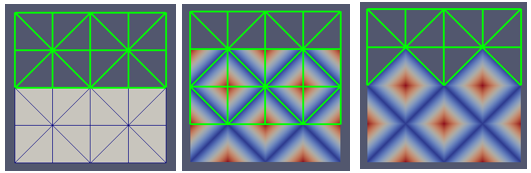
\includegraphics[width=0.5\textwidth]{mpi_indset.png}}
\caption{Steps to distributed adapt: (left) non-ghosted partitions (mid)
add ghost layers, compute independent set (right)
trim away non-owned ghosts}\vspace*{-6pt}
\label{fig:mpi_indset}
\end{figure}

During each adaptation pass, we do what is possible without a ghost
layer first. Typically, this means measuring edge lengths and determining
whether any of them are too long or two short.
Then a ghost layer is constructed and possible operations are evaluated
as described above and an independent set is chosen as described in
Section \ref{sec:indset}.
Once an independent set has been chosen, we return to an element-based
partitioning, but one which is altered such that cavities in the independent
set reside on one MPI rank.
At that point, the code can proceed to apply the cavity modifications
and produce a new local mesh structure without further communication
because shared entities are not modified.
Figure \ref{fig:mpi_indset} illustrates this process at a simple partition boundary,
in the case of selecting which mesh vertices ought to be collapsed.

The tracking of parallel connectivity in our code is based first on global
IDs for the entities.
By the definition of our partitioning, new cavity entities are only created
inside the MPI rank which owns the cavity, so we assign their ownership
to that rank.
We can also take the intersection of entities that stayed the same
(not in cavities) and are owned.
Together these numbers give a count of how many entities in the new mesh are owned
by the local MPI rank.
A simple \texttt{MPI\_Exscan} function call converts local counts into
global numbers for owned copies.
There are still non-owned copies which do not know their global ID, but they
are by definition entities which stayed the same, so we can use the
communication instruments of the old mesh to synchronize their IDs.

Combined with the independent set selection mechanism, this results
in a mesh adaptation method which is unaffected by partition boundaries,
in the sense that the decision process of what modifications to apply
is not influenced by the partition.
The resulting algorithm is also deterministic,
in that its output is the same regardless of the order of
execution of shared memory threads and MPI processes.
Its output is independent
of ordering so long as global IDs are independent of ordering.
Most other parallel adaptation implementations that we know of explicitly
consider interior modifications first, followed by a repartitioning that
allows consideration and modification of the near-boundary mesh
\cite{loseille2015parallel,de1999parallel}, making them
partitioning-dependent.

\section{On-Node Parallelism}

\subsection{Inter-Thread Communication}
\label{sec:itc}

Second half of the PCU paper describes how we were able to use
threading without rewriting everything.

\subsection{Parallel For Loops}
\label{sec:parallel_for}

Omega\_h content on how to do threading and GPUs properly
when the code is rewritten.

\section{Determinism}
\label{sec:determinism}

Discuss things done by Omega\_h to achieve
determinism on heterogeneous architectures.

\subsection{Adjacency Inversion}

The key algorithms Ben and I came up with go here.

\subsection{Order-Independent Sums}

%%% Local Variables:
%%% mode: latex
%%% TeX-master: t
%%% End:

